% Exam Template for UMTYMP and Math Department courses
%
% Using Philip Hirschhorn's exam.cls: http://www-math.mit.edu/~psh/#ExamCls
%
% run pdflatex on a finished exam at least three times to do the grading table on front page.
%
%%%%%%%%%%%%%%%%%%%%%%%%%%%%%%%%%%%%%%%%%%%%%%%%%%%%%%%%%%%%%%%%%%%%%%%%%%%%%%%%%%%%%%%%%%%%%%

% These lines can probably stay unchanged, although you can remove the last
% two packages if you're not making pictures with tikz.
\documentclass[11pt]{exam}
\RequirePackage{amssymb, amsfonts, amsmath, latexsym, verbatim, xspace, setspace}
\RequirePackage{tikz, pgflibraryplotmarks}

% By default LaTeX uses large margins.  This doesn't work well on exams; problems
% end up in the "middle" of the page, reducing the amount of space for students
% to work on them.
\usepackage[margin=1in]{geometry}
%\usepackage{tkz-euclide}
\usepackage{multicol}
\usepackage{graphicx}
\usepackage{tikz,pgfplots}
\usepackage{listings}
\usepackage{pdfpages}
\usepackage{minitoc} %% Required
\usepackage{tabularx}

% Here's where you edit the Class, Exam, Date, etc.
\newcommand{\class}{Calculus I}
\newcommand{\term}{Fall 2020}
\newcommand{\examnum}{Lab 1: Review of High School Math}
\newcommand{\examdate}{August 20, 2020}

% For an exam, single spacing is most appropriate
\singlespacing
% \onehalfspacing
% \doublespacing

% For an exam, we generally want to turn off paragraph indentation
\parindent 0ex

\begin{document} 
	
	% These commands set up the running header on the top of the exam pages
	\pagestyle{head}
	\firstpageheader{}{}{}
	\runningheader{\class}{\examnum\ - Page \thepage\ of \numpages}{\examdate}
	\runningheadrule
	
	\begin{flushright}
		\begin{tabular}{p{2.8in} r l}
			\textbf{\class} & \textbf{Name (Print):} & \makebox[2in]{\hrulefill}\\
			\textbf{\term} &&\\
			\textbf{\examnum} &&\\
			%\textbf{\examdate} &&\\
			%\textbf{Due Date: \duedate}
			%\textbf{Time Limit: \timelimit} & Teaching Assistant & \makebox[2in]{\hrulefill}
		\end{tabular}\\
	\end{flushright}
	
Show all your work, cite your sources, and type your answers for full credit.\\

Materials needed: tape measure, scissors, ruler or phone measurement app, lev-o-gage or suncalc phone app, thermometer or Google
	
	\rule[1ex]{\textwidth}{.1pt}
	
	\setlength{\columnsep}{0.5 in}
	
	\begin{questions}
		
		\addpoints
		
		\question[5] \textbf{Review of Rates and Unit Conversion:}
		You are out and about frolicking in nature, when you suddenly see dark clouds. You see lighting strike some distance off, and exactly 7.3 seconds later you hear thunder. How far away was the lightning strike? Provide your answer in miles.   If you don't have the speed of sound memorized (who doesn't?) you can feel free to Google it.
		
		\question[5] \textbf{Review of Trigonometry and Problem Solving:}
		How tall is the steeple on top of McClain from the ground?  If you are doing this lab at home, pick a tall object near your house, get the suncalc app on your phone, and measure the shadow of that object at two different times, marking the angle of the sun each time.
		
		\question[5] \textbf{Review of Linear Functions.:}
		Use two points on a thermometer to find an equation that converts temperature from F to C.  If you do not have an alcohol or mercury thermometer handy, use Google to convert two temperatures from Fahrenheit to Celsius.
		
		\question[5] \textbf{Review of Geometry and Trigonometry:}
		
		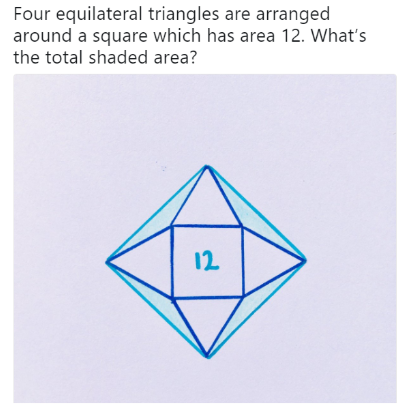
\includegraphics[width=4 in]{images/geo.png}
		
		\newpage
		
		\question[5] \textbf{Review of geometry and prelude to optimization:}
		Grab a piece of computer paper. With this paper, cut squares out of each of the corners and make a box by folding up the edges. How much should you cut out to give you the maximum volume? You will need a ruler, scissors, and tape.
		
		This question will be graded on how close you come to the optimum volume, your communication of your solution, and your perceived effort.
		
		
		
		
	\end{questions}
	
\end{document}
